\documentclass[slidestop,compress,mathserif]{beamer}
%\documentclass[slidestop,compress,mathserif,handout]{beamer}

%\documentclass[xcolor=dvipsnames,handout]{beamer}
%\documentclass[xcolor=dvipsnames]{beamer}

%\documentclass[handout]{beamer}

%%% To get rid of solutions on handouts:
\newcommand{\soln}[1]{\textit{\textcolor{darkGray}{#1}}}				% For slides
%\newcommand{\soln}[1]{ }	% For handouts

% to get pausing to work properly on slides
\newcommand{\hide}[1]{#1}	% For slides
%\newcommand{\hide}[1]{ }	% For handouts


%\usepackage{multicol}
\usepackage{amsfonts}
%\usepackage[pdftex,dvipsnames]{color}
\usepackage{graphicx}
\usepackage{subfigure}
%\usepackage{picinpar}
\usepackage{pifont}
\usepackage{pgf,pgfarrows,pgfnodes}
%\usepackage{wasysym,manfnt,phaistos,empheq}
\usepackage[english]{babel}
\usepackage{pgfpages}
\usepackage{natbib}
\usepackage{hyperref}
\usepackage{multimedia}
%\usepackage{amsfonts,amstext,amssymb,amsbsy,amsopn,amsthm,eucal,latexsym,mathrsfs}
\usepackage{amsmath,amsfonts,amstext,amssymb,amsbsy,amsopn,amsthm,eucal,latexsym,mathrsfs}
\usepackage{ulem}
\usepackage{setspace}
\usepackage{array}
%\usepackage{rotating}
\usepackage{multirow}
\usepackage{verbatim}
\usepackage{multicol}

\setbeamertemplate{navigation symbols}{}

%\usepackage{tikz}
%\usetikzlibrary{arrows,shapes,trees,backgrounds}


%\setbeameroption{show notes on second screen}
%\setbeameroption{show notes}
%\setbeameroption{show only notes}

\definecolor{links}{HTML}{2A1B81}
\hypersetup{colorlinks,linkcolor=,urlcolor=links}

\newtheorem*{principle}{Inscrutibility Principle}
\newtheorem*{punchline}{Punch Line}
\newtheorem{defn}{Definition}

\definecolor{Scarlet}{RGB}{140,17,17}
\definecolor{VassarRed}{RGB}{128,0,0}

% "dinglist" environment
  \renewenvironment{dinglist}[2][blue]
  {\begin{list}{\textcolor{blue}{\ding{#2}}}{}}{\end{list}}
  % Symbol definitions for these lists
  \newcommand{\DingListSymbolA}{43}
  \newcommand{\DingListSymbolB}{243}
  \newcommand{\DingListSymbolC}{224}
  \newcommand{\DingListSymbolD}{219}
  \newcommand{\DingListSymbolCheck}{52}
  \newcommand{\DingListSymbolCross}{56}


  \newenvironment{ballotenv}
{\only{%
\setbeamertemplate{itemize item}{\ding{45}}%
\setbeamertemplate{itemize subitem}{\ding{46}}%
\setbeamertemplate{itemize subsubitem}{\ding{46}}}} {}
\setbeamertemplate{itemize item}{\ding{49}}
\setbeamertemplate{itemize subitem}{\ding{47}}
\setbeamertemplate{itemize subsubitem}{\ding{47}}


%User defined colors: See colors section
\xdefinecolor{oiBlue}{rgb}{0.15, 0.35, 0.55}
\xdefinecolor{gray}{rgb}{0.5, 0.5, 0.5}
\xdefinecolor{darkGray}{rgb}{0.3, 0.3, 0.3}
\xdefinecolor{darkerGray}{rgb}{0.2, 0.2, 0.2}
\xdefinecolor{rubineRed}{rgb}{0.89,0,0.30}
\xdefinecolor{linkCol}{rgb}{0.11,0.49,0.95}	
\xdefinecolor{irishGreen}{rgb}{0,0.60,0}	
\xdefinecolor{darkturquoise}{rgb}{0.44, 0.58, 0.86}
\definecolor{lightGreen}{rgb}{0.533,0.765,0.42}
\xdefinecolor{Regalia}{HTML}{522D80}
\xdefinecolor{ClemsonOrange}{HTML}{EA6A20}

\definecolor{duke@LightGrey}{RGB}{200,200,200}\definecolor{DarkGreen}{RGB}{0,100,0}
\definecolor{Oranges}{RGB}{255,127,0}
\definecolor{LightGray}{RGB}{211,211,211}

%\setbeamertemplate{footline}{%
%  \raisebox{5pt}{\makebox[\paperwidth]{\hfill\makebox[10pt]{\scriptsize\insertframenumber}}}}

\setbeamercolor{equation background}{fg=black,bg=duke@LightGrey}
  % Boxed equation
  \newcommand{\eqbox}[2][0.6]{%
  \centerline{
  \begin{beamerboxesrounded}[lower=equation background,width=#1\hsize,shadow=true]{}
\parbox{#1\hsize}{%
      \[
        \textcolor{black} {#2}
      \]}
  \end{beamerboxesrounded}
}}

\AtBeginSection[] {
  \begin{frame}<beamer>\frametitle{Outline}
    \tableofcontents[currentsection,hideothersubsections]
  \end{frame}
}
%
%
%\AtBeginSubsection[] {
%  \begin{frame}<beamer>\frametitle{Outline}
%    \tableofcontents%[currentsection,currentsubsection]
%  \end{frame}
%}

%\usecolortheme[RGB={82,45,128}]{structure}
%\usecolortheme[RGB={162,80,22}]{structure}
\usecolortheme[RGB={128,0,0}]{structure}
\usetheme[secheader]{Boadilla}
%\usetheme[height=7mm]{Rochester}
%\usetheme{Copenhagen}
%\usetheme{Antibes}
%\usecolortheme{seahorse}
%\usecolortheme{crane}
%\usecolortheme{rose}
%\usefonttheme[onlylarge]{structurebold}
%\usefonttheme[onlymath]{serif}



\def\diag{{\rm diag}}


\def\E{\mathbb{E}}
\def\Prob{\mathbb{P}}
\def\argmin{{\rm argmin}}
\def\argmax{{\rm argmax}}
\def\Def{\stackrel{def}{=}}


\newtheorem{assumption}{Assumptions}
\newtheorem*{proposition}{Proposition}
\newtheorem*{remark}{Remark}



%\setbeamercolor{disc title}{bg=oiBlue!40!white!60,fg=blue}
\setbeamercolor{disc body}{bg= Regalia!20!white!80,fg= Regalia!80!black!90}

\setbeamercolor{clicker ungraded title}{bg=irishGreen!80!white!50,fg=irishGreen!30!black!90}
\setbeamercolor{clicker ungraded body}{bg=irishGreen!20!white!80,fg=irishGreen!30!black!90}

\setbeamercolor{clicker review title}{bg=gray!80!white!80,fg=oiBlue!80!black!90}
\setbeamercolor{clicker review body}{bg=gray!30!white!90,fg=oiBlue!80!black!90}

\setbeamercolor{code body}{bg=gray!20!white!80,fg=black}


% Custom commands
\newcommand{\degree}{\ensuremath{^\circ}}
\newcommand{\Note}[1]{
\rule{2.5cm}{0.25pt} \\ \textit{\scriptsize {\textcolor{rubineRed}{Note:} \textcolor{gray}{#1}}}}
\newcommand{\ct}[1]{
\vfill
{\tiny #1}}
\newcommand{\Remember}[1]{\textit{\scriptsize{\textcolor{orange}{Remember:} \textcolor{gray}{#1}}}}
\newcommand{\red}[1]{\textit{\textcolor{rubineRed}{#1}}}
\newcommand{\pink}[1]{\textit{\textcolor{rubineRed!90!white!50}{#1}}}
\newcommand{\green}[1]{\textit{\textcolor{irishGreen}{#1}}}
\newcommand{\webURL}[1]{\urlstyle{same}\textit{\textcolor{linkCol}{\url{#1}}} }
\newcommand{\webLink}[2]{\href{#1}{\textcolor{linkCol}{{#2}}}}
\newcommand{\mail}[1]{\href{mailto:#1}{\textit{\textcolor{linkCol}{#1}}}}
\newcommand{\hl}[1]{\textit{\textcolor{oiBlue}{#1}}}
\newcommand{\hlGr}[1]{\textit{\textcolor{lightGreen}{#1}}}
\newcommand{\mathhl}[1]{\textcolor{oiBlue}{\ensuremath{#1}}}
\newcommand{\ex}[1]{\textcolor{blue}{{{\small (#1)}}}}
\newcommand{\disc}[1]{
\begin{beamerboxesrounded}[shadow = true, lower = disc body, upper = disc title]{}
#1
\end{beamerboxesrounded}
}

\newcommand{\cl}[1]{
\begin{beamerboxesrounded}[shadow = true, lower = clicker ungraded body, upper = clicker ungraded title]{Question}
$\:$ \\
#1
\end{beamerboxesrounded}
}

\newcommand{\clR}[1]{
\begin{beamerboxesrounded}[shadow = true, lower = clicker review body, upper = clicker review title]{\red{Review question} }
$\:$ \\
#1
\end{beamerboxesrounded}
}

\newcommand{\formula}[2]{
\begin{beamerboxesrounded}[shadow = true, lower = white, upper = clicker review body]{#1}
#2
\end{beamerboxesrounded}
$\:$ \\
}

\newenvironment{twocol}[4]{
\begin{columns}[c]
\column{#1\textwidth}
#3
\column{#2\textwidth}
#4
\end{columns}
}


\newenvironment{slot}[2]{
\begin{array}{c}
\underline{#1} \\
#2
\end{array}
}

\newcommand{\pr}[1]{
\left( #1 \right)
}

\newcommand{\solnMult}[1]{
\item[] \vspace{-0.59cm}
\only<beamer| beamer:1>{\item #1}
\soln{\only<2->{\item \red{#1}}}
}

%\newcommand{\codechunk}[1]{
%\begin{beamerboxesrounded}[shadow = true, lower = code body]{}
%{\small #1}
%\end{beamerboxesrounded}
%}

% Change margin

\newenvironment{changemargin}[2]{%
\begin{list}{}{%
\setlength{\topsep}{0pt}%
\setlength{\leftmargin}{#1}%
\setlength{\rightmargin}{#2}%
\setlength{\listparindent}{\parindent}%
\setlength{\itemindent}{\parindent}%
\setlength{\parsep}{\parskip}%
}%
\item[]}{\end{list}}

% Footnote

\long\def\symbolfootnote[#1]#2{\begingroup%
\def\thefootnote{\fnsymbol{footnote}}\footnote[#1]{#2}\endgroup}

% Commands from the book
\newenvironment{data}[1]{\texttt{#1}}{}
\newenvironment{var}[1]{\texttt{#1}}{}
\newenvironment{resp}[1]{\texttt{#1}}{}






%%%%%%%%%%%%%%%%%%%%%%%%%%%%%%%%%%%%%%%%%%%%%%%%%%%%%%%%%%%%%%%%%%%%%%%%%%%%%%%%%%%%%%%%%%%%%%%

\title[Chapter 6 part 1]{Chapter 6 part 1}
\subtitle{Jointly Distributed Random Variables}

%%%%%%%%%%%%%%%%%%%%%%%%%%%%%%%%%%%%%%%%%%?%%%%%%%%%%%%%%%%%%%%%%%%%%%%%%%%%%%%%%%%%%%%%%%%%%%%%


\author[Jingchen (Monika) Hu] % (optional, use only with lots of authors)
{Jingchen (Monika) Hu}
% - Give the names in the same order as the appear in the paper.
% - Use the \inst{?} command only if the authors have different
%   affiliation.

\institute[Vassar] % (optional, but mostly needed)
{Vassar College}
% - Use the \inst command only if there are several affiliations.
% - Keep it simple, no one is interested in your street address.

\date[MATH 241] % (optional, should be abbreviation of conference name)
{MATH 241}
% - Either use conference name or its abbreviation.
% - Not really informative to the audience, more for people (including
%   yourself) who are reading the slides online

\subject{MATH 241}
% This is only inserted into the PDF information catalog. Can be left
% out.



% If you wish to uncover everything in a step-wise fashion, uncomment
% the following command:

%\beamerdefaultoverlayspecification{<+->}



\begin{document}

%\begin{frame}%[plain]
%
\includegraphics[width = \textwidth]{figures/2015DukeNCAA}
%\end{frame}
%
%{ % all template changes are local to this group.
%\addtocounter{framenumber}{-1}
%    \setbeamertemplate{navigation symbols}{}
%    \begin{frame}[plain]
%        \begin{tikzpicture}[remember picture,overlay]
%            \node[at=(current page.center)] {
%                
\includegraphics[width=1.25\paperwidth]{figures/2015DukeNCAA}
%            };
%        \end{tikzpicture}
%     \end{frame}
%}

%%%%%%%%%%%%%%%%%%%%%

% Title Page

\begin{frame}%[plain]
\titlepage
\end{frame}


%%%%%%%%%%%%%%%%%%%%%%
%\addtocounter{framenumber}{-1}
%
%\begin{frame}\frametitle{Annoucement}
%
%\begin{itemize}
%%\item HW7: \red{due now!}
%\item HW8: \red{due Tuesday, Nov 20th}
%
%
%\vspace{0.5cm}
%\item Course evaluation open tomorrow.
%  \begin{itemize}
%  \item Activate between 11/14 - 12/3.
%  \item If response rate $\geq 80\%$, drop the lowest quiz.
%  \end{itemize}
%
%\vspace{0.5cm}
%\item Next quiz: Tuesday, Nov 18th\\
%  \begin{itemize}
%  \item Topic: function of a continuous random variable, i.e., find $f_Y(y)$ where $Y = g(X)$.
%  %\item To prepare: do homework questions in Chapter 5: 37, 39, 40, TE29
%  \end{itemize}
%
%
%%\item Midterm: Tuesday, Feb 25th
%%\begin{itemize}
%%\item Close book, in class exam (75 min)
%%\item ONE page cheat sheet {\bf made by yourself} (A4 size)
%%\item Calculators are allowed, but not cell phones, tablets or laptops
%%\end{itemize}
%
%\end{itemize}
%
%
%\end{frame}
%

%
%%%%%%%%%%%%%%%%%%%%%%
\begin{frame}{Outline}
%\tableofcontents[hideallsubsections,pausections]
\tableofcontents[hideallsubsections]
\end{frame}

%%%%%%%%%%%%%%%%%%%%%%%%%%%%%%%%%%%%%%%%%%
%\begin{frame}\frametitle{Recap}
%
%Distribution (pdf) of a function of a continuous random variable $X$: if function $g(x)$ is
%\begin{enumerate}
%\item monotonic,
%\item differentiable,
%\end{enumerate}
%\pause
%on the range of $X$, then the random variable defined by $Y = g(X)$ has pdf
%\[ f_Y ( y ) = f_X( x )  \left|\frac{dx}{dy}\right| \]
%
%\pause
%\begin{itemize}
%\item When conditions are not satisfied, \pause
%  \begin{enumerate}[(1)]
%  \item  Identify the range of $Y$. \pause
%  \item Find cdf $F_Y(y)$ as a function of $F_X(\cdot)$, for any $y$ in the range of $Y$. \pause
%  \item Take derivative to get $f_Y(y)$. \pause
%  \item Note that for any $y$ not in the range of $Y$, $f_Y(y) = 0$.
%  \end{enumerate}
%\end{itemize}
%
%\end{frame}
%




%%%%%%%%%%%%%%%%%%%%%
%\begin{frame}{Outline}
%%\tableofcontents[hideallsubsections,pausections]
%\tableofcontents[hideallsubsections]
%\end{frame}



%%%%%%%%%%%%%%%%%%%%%%%%%%%%%%%%%%%%%%%%%%
\section{Joint distribution}
%%%%%%%%%%%%%%%%%%%%%%%%%%%%%%%%%%%%%%%%%%
\begin{frame}
\frametitle{Joint cdf}

\begin{defn}
We have a pair of random variables (either discrete or continuous) $X$ and $Y$.
The \hl{joint cumulative probability distribution function} of $X$ and $Y$ is defined by
\vspace{-0.3cm}
\begin{align*}
F_{X, Y}(x,y) &= P[ X \leq x, Y \leq y ] \\
 &= P[ (X,Y)\text{ lies south-west of the point }(x,y) ]
\end{align*}
\end{defn}

\vspace{-0.7cm}
\begin{center}
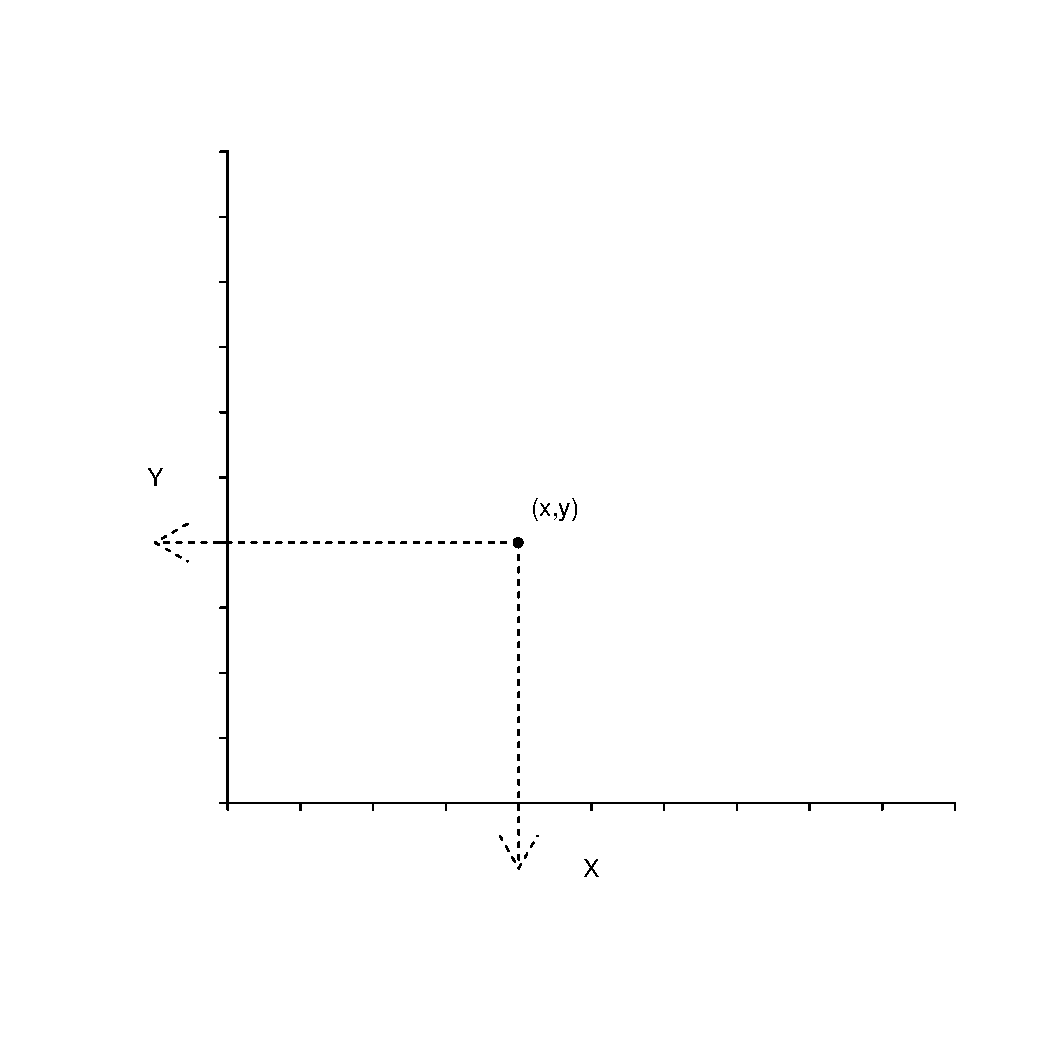
\includegraphics[width=0.5\textwidth]{figures/cdf.pdf}
\end{center}


\end{frame}


%%%%%%%%%%%%%%%%%%%%%%%%%%%%%%%%%%%%%%%%%%
\begin{frame}
\frametitle{Properties of joint cdf}

\begin{itemize}
\item For one random variable: marginal cdf
\[ F_X(x) =   F_{X, Y}(x, \infty)\]
\[ F_X(x) = P(X \leq x) = P(X \leq x, Y \leq \infty) =  F_{X, Y}(x, \infty)\]
\[ F_Y(y) =   F_{X, Y}(\infty, y)\]
\[ F_Y(y) = P(Y \leq y) = P(X \leq \infty, Y \leq y) =  F_{X, Y}(\infty, y)\]


\item Joint probabilities
\[ P(X > x, Y > y) = 1 - F_X(x) - F_Y(y) + F_{X, Y}(x, y)\]
\end{itemize}


\end{frame}

%%%%%%%%%%%%%%%%%%%%%%%%%%%%%%%%%%%%%
\begin{frame}\frametitle{}


\cl{Use joint cdf $F(x, y)$ to represent $P(x_1 < X \leq x_2, y_1 < Y \leq y_2)$.}

\begin{enumerate}[(a)]
\solnMult{$F(x_2, y_2) + F(x_1, y_1) - F(x_1, y_2) - F(x_2, y_1)$}
\item $F(x_2, y_2) - F(x_1, y_1) - F(x_1, y_2) - F(x_2, y_1)$
\item $F(x_2, y_2) - F(x_1, y_1)$
\item none of the above
\end{enumerate}



\end{frame}


\begin{frame}
\frametitle{Marginal Distributions}

Note that the column and row sums are the distributions of $B$ and $W$ respectively.

{\footnotesize
\[P(B=b) = P(B=b,W=0)+P(B=b,W=1)+P(B=b,W=2)\]
\[P(W=w) = P(B=0,W=w)+P(B=1,W=w)+P(B=2,W=w)\]
}

These are the \emph{marginal} distributions of $B$ and $W$. In general,
\[ P(X=x) = \sum_y P(X=x,Y=y) = \sum_y P(X=x \mid Y=y)P(Y=y)\]

\end{frame}


%%%%%%%%%%%%%%%%%%%%%%%%%%%%%%%%%%%%%%%%%


\begin{frame}
\frametitle{Conditional Distribution}

Conditional distributions are defined as we have seen previously with

\[ P(X=x \mid Y=y) = \frac{P(X=x,Y=y)}{P(Y=y)} = \frac{\text{joint pmf}}{\text{marginal pmf}} \]

\end{frame}

\begin{frame}
\cl{Draw two socks at random, without replacement, from a drawer full of twelve colored socks:
6 black, 4 white, 2 purple. Let $B$ be the number of Black socks, $W$ the number of White socks drawn. Find the pmf for white socks given no black socks were drawn.}

\twocol{0.4}{0.6}{
\vspace{-8mm}
\begin{center}
\renewcommand{\arraystretch}{1.5}
\begin{tabular}{cc|c|c|c|c}
\multicolumn{2}{c}{} & \multicolumn{3}{c}{W} & \multicolumn{1}{c}{} \\
  &       & 0               & 1               & 2              &                 \\ \cline{2-6}
  & ~~0~~ & $\frac{1}{66}$  & $\frac{8}{66}$  & $\frac{6}{66}$ & $\frac{15}{66}$ \\ \cline{2-6}
B & ~~1~~ & $\frac{12}{66}$ & $\frac{24}{66}$ & $0$            & $\frac{36}{66}$ \\ \cline{2-6}
  & ~~2~~ & $\frac{15}{66}$ & $0$             & $0$            & $\frac{15}{66}$ \\ \cline{2-6}
  &       & $\frac{28}{66}$ & $\frac{32}{66}$ & $\frac{6}{66}$ & $\frac{66}{66}$ \\
\end{tabular}
\end{center}

}{
%\invisible{
\pause
\vspace{-5mm}
\begin{align*}
& P(W=w \mid B=0) \\
= & \frac{P(W=w, B=0)}{P(B=0)}\\
= & \begin{cases}
\left.\frac{1}{66}\right/\frac{15}{66} = \frac{1}{15} &\text{if $W=0$}\\
\left.\frac{8}{66}\right/\frac{15}{66} = \frac{8}{15} &\text{if $W=1$}\\
\left.\frac{6}{66}\right/\frac{15}{66} = \frac{6}{15} &\text{if $W=2$}\\
\end{cases}
\end{align*}
%}
}

\end{frame}


%%%%%%%%%%%%%%%%%%%%%%%%%%%%%%%%%%%%%%%%%%%
%\section{Joint distribution of two continuous random variables}
%%%%%%%%%%%%%%%%%%%%%%%%%%%%%%%%%%%%%%%%%%

\begin{frame}
\frametitle{Joint distribution of two continuous random variables}

\vspace{-0.2cm}
\begin{defn}
Random variables $X$ and $Y$ are \hl{jointly continuous} if there exists a function $f(x, y)$ such that
\begin{enumerate}
%\vspace{0.2cm}
\item Non-negative $f(x, y) \geq 0$, for any $x, y \in \mathbb{R}$, and
%\vspace{0.2cm}
\item $\int_{-\infty}^{\infty} \int_{-\infty}^{\infty} f(x,y) ~dx~dy = 1$.
\end{enumerate}
%\vspace{0.2cm}
$f_{X, Y}(x, y)$ is called the \hl{joint probability density function} of $X$ and $Y$.
\end{defn}
\vspace{-0.2cm}

\begin{itemize}
\item 
For any set $C \subset \mathbb{R}^2$,
\[ P[(X, Y) \in C] = \iint_{(x, y) \in C} f(x,y) ~dx~dy\]
\vspace{-0.2cm}
\item 
Connection between joint pdf and joint cdf
\vspace{-0.2cm}
\[ F(a,b) = P(X\leq a,Y\leq b) = \int_{-\infty}^b \int_{-\infty}^a f(x,y) ~dx~dy \] \vspace{-0.2cm}
\[f(x,y) = \frac{\partial^2}{\partial x \partial y} F(x,y)\]

\end{itemize}


\end{frame}


%%%%%%%%%%%%%%%%%%%%%%%%%%%%%%%%%%%%%%%%%%
\begin{frame}
\frametitle{Marginal pdfs}

Marginal probability density functions are defined in terms of ``integrating out'' one of the random variables.

\[ f_X(x) = \int_{-\infty}^\infty f(x,y)~dy \]
\[ f_Y(y) = \int_{-\infty}^\infty f(x,y)~dx \]

%Previously we defined independence in terms of $E(XY) = E(X)E(Y) \Rightarrow$ $X$ and $Y$ are independent. This is equivalent in the joint case of $f(x,y) = f_X(x)f_Y(y) \Rightarrow$ $X$ and $Y$ are independent.

\end{frame}

%%%%%%%%%%%%%%%%%%%%%%%%%%%%%%%%%%%%%%%%%%
\begin{frame}\frametitle{}
\cl{Which of the following can be obtained if the joint pdf $f_{X, Y}(x, y)$ is known?}

\begin{enumerate}[(a)]
\item Joint cdf $F_{X, Y}(x, y)$
\item Marginal cdfs $F_X(x), F_Y(y)$.
\item Expected values $E[X], E[Y]$.
\solnMult{all above}
\end{enumerate}

\end{frame}


%%%%%%%%%%%%%%%%%%%%%%%%%%%%%%%%%%%%%%%%%%%
%\section{Examples of joint distributions of continuous random variables}
%%%%%%%%%%%%%%%%%%%%%%%%%%%%%%%%%%%%%%%%%%
%%%%%%%%%%%%%%%%%%%%%%%%%%%%%%%%%%%%%%%%%%
\begin{frame}\frametitle{Recap}

Joint cdf of two random variables $X$ and $Y$:
\[ F_{X, Y}(x,y) = P[ X \leq x, Y \leq y ], -\infty < x, y < \infty \]
%\vspace{-0.3cm}
\begin{itemize}
\item Probability of $(X, Y)$ in a rectangle
\[P(x_1 < X \leq x_2, y_1 < Y \leq y_2)\]\[ = F(x_2, y_2) + F(x_1, y_1) - F(x_1, y_2) - F(x_2, y_1)\]
\item Marginal cdfs
\[ F_X(x) = F_{X, Y}(x, \infty), \quad F_Y(y) =  F_{X, Y}(\infty, y)\]
\end{itemize}

\end{frame}

%%%%%%%%%%%%%%%%%%%%%%%%%%%%%%%%%%%%%%%%%%
\begin{frame}%\frametitle{Recap}

{\bf Joint distribution of two discrete random variables}
\begin{itemize}
\item Joint pmf
\[p_{X, Y}(x, y) = P(X=x,Y=y) \]
\item Marginal pmfs
\[p_X(x) = \sum_{y: p(x, y) > 0} p_{X, Y}(x,y), \quad p_Y(y) = \sum_{x: p(x, y) > 0} p_{X, Y}(x,y)  \]
\end{itemize}

{\bf Joint distribution of two continuous random variables }
\begin{itemize}
\item Joint pdf
  \begin{itemize}
  \item Non-negative $f_{X, Y}(x, y) \geq 0$, for any $x, y \in \mathbb{R}$
  \item $\int_{-\infty}^{\infty} \int_{-\infty}^{\infty} f_{X, Y}(x,y) ~dx~dy = 1$
  \item For any set $C \subset \mathbb{R}^2$,
  \[ P[(X, Y) \in C] = \iint_{(x, y) \in C} f_{X, Y}(x,y) ~dx~dy\]
  \end{itemize}
\item Marginal pdfs
\[ f_X(x) = \int_{-\infty}^\infty f_{X, Y}(x,y)~dy, \quad f_Y(y) = \int_{-\infty}^\infty f_{X, Y}(x,y)~dx \]
\end{itemize}


\end{frame}


%%%%%%%%%%%%%%%%%%%%%%%%%%%%%%%%%%%%
\begin{frame}%\frametitle{Distribution of a function of a discrete random variable}

\cl{Let $X$ have a Bin$(n, p)$ distribution. What's the pmf of $Y = 2X$?}

\begin{enumerate}[(a)]
\item $f_Y(y) = {2n \choose y}(2p)^y (1-2p)^{2n - y}$ for any $y \in \{0, 2, 4, \ldots, 2n\}$
\item $f_Y(y) = {2n \choose y}p^y (1-p)^{2n - y}$ for any $y \in \{0, 1, 2, \ldots, 2n\}$
\solnMult{$f_Y(y) = {n \choose y/2}p^{\frac{y}{2}} (1-p)^{n - \frac{y}{2}}$ for any $y \in \{0, 2, 4, \ldots, 2n\}$}
\item $f_Y(y) = \frac{1}{2}{n \choose y/2}p^{\frac{y}{2}} (1-p)^{n - \frac{y}{2}}$ for any $y \in \{0, 2, 4, \ldots, 2n\}$
\end{enumerate}

%\invisible{
\pause
\[ f_Y(y) = P(Y = y) = P\left(X = \frac{y}{2}\right) = f_X\left(\frac{y}{2}\right) \]

%}

\end{frame}



%%%%%%%%%%%%%%%%%%%%%%
%\begin{frame}{Outline}
%%\tableofcontents[hideallsubsections,pausections]
%\tableofcontents[hideallsubsections]
%\end{frame}


%%%%%%%%%%%%%%%%%%%%%%%%%%%%%%%%%%%%%%%%%%%
%\section{Examples of joint distributions of continuous random variables}
%%%%%%%%%%%%%%%%%%%%%%%%%%%%%%%%%%%%%%%%%%




%%%%%%%%%%%%%%%%%%%%%%%%%%%%%%%%%%%%%%%%%%
\begin{frame}
\cl{Let X and Y have the following joint pdf
\[ f(x,y) = \begin{cases}
    \frac{2}{9} & \text{ for } x\geq 0, y \geq 0 \text{ and } x+y \leq 3 \\
    0           & \text{otherwise}
\end{cases}
 \]
Find the marginal pdf of $Y$.}
\twocol{0.3}{0.7}
{
\begin{center}
    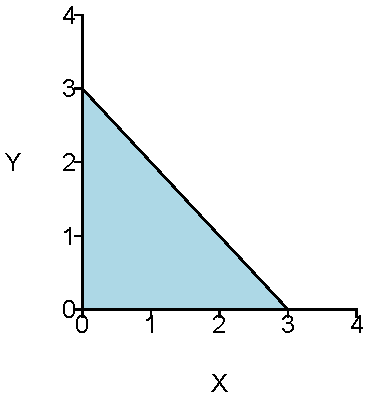
\includegraphics[width=\textwidth]{figures/triangle2.pdf}
\end{center}
}
{
%\invisible{
\vspace{-36pt}
\[
f_Y(y) = \begin{cases}
    \uncover<2>{\frac{2}{9}(3-y) & \text{ for } y\in [0,3] \\}
    \uncover<2>{0           & \text{otherwise}}
\end{cases}
\]
%}
}

\end{frame}
%%%%%%%%%%%%%%%%%%%%%%%%%%%%%%%%%%%%%%%%%%



\begin{frame}


\twocol{0.5}{0.5}
{
\cl{Let $f(x,y) = c x^2 y$ for $x^2 \leq y \leq 1$. Find:
\begin{enumerate}[(a)]
\item $c$
\item $P[ X \geq Y ]$
\item $f_X(x)$ and $f_Y(y)$
\end{enumerate}
\vfill
}
}
{
\begin{center}
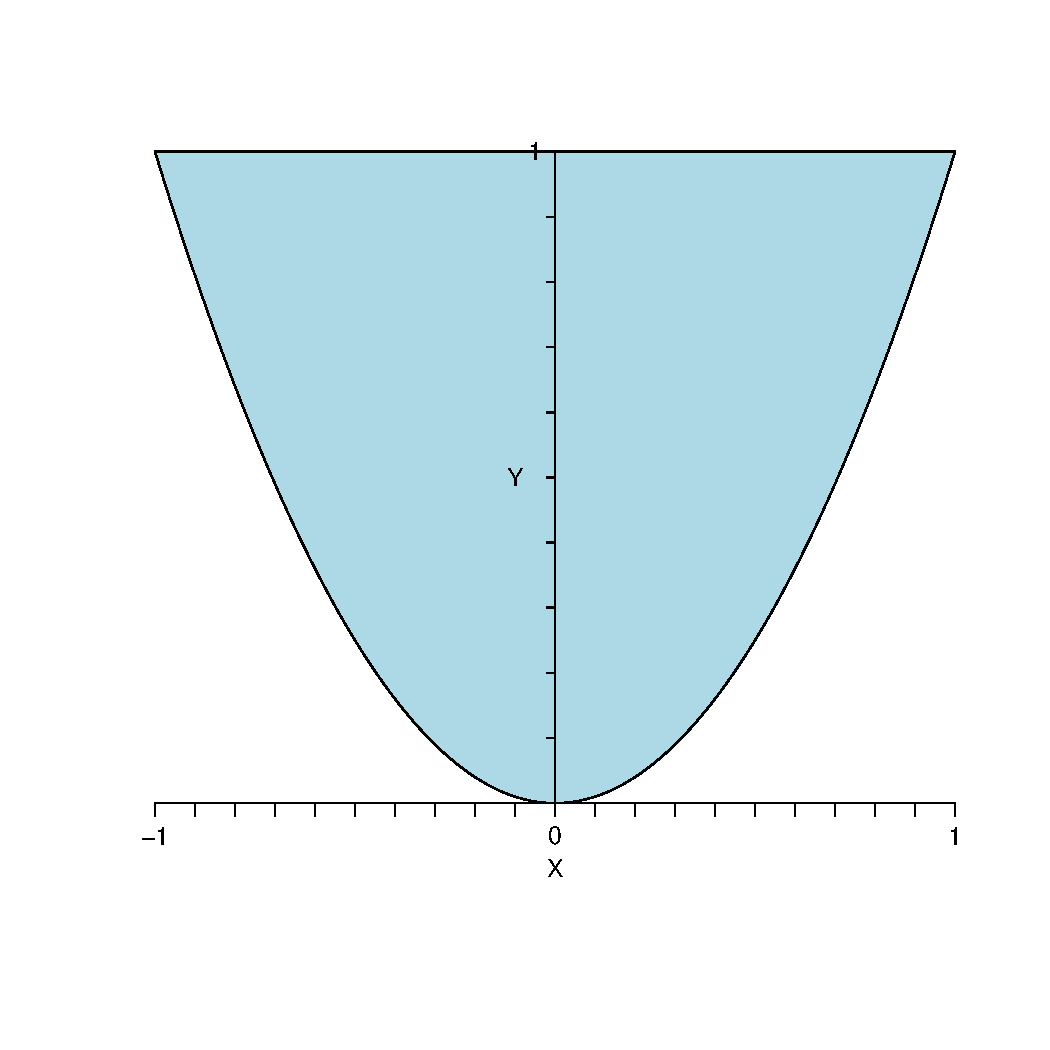
\includegraphics[width=\textwidth]{Figures/ex3-range.pdf}
\end{center}
}
\end{frame}

%%%%%%%%%%%%%%%%%%%%%%%%%%%%%%%%%%%%%%%%%%

\begin{frame}

Let $f(x,y) = c x^2 y$ for $x^2 \leq y \leq 1$, we can rewrite the bounds as
\uncover<2->{\[0\leq y \leq 1, \quad -\sqrt{y} \leq x \leq \sqrt{y}\]}
\twocol{0.3}{0.7}
{
\begin{center}
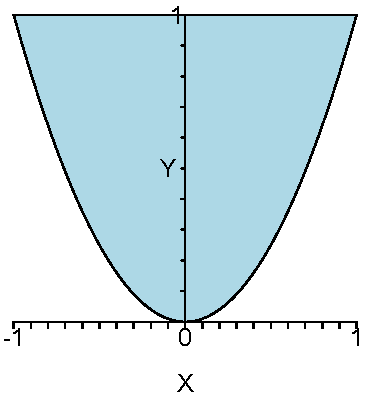
\includegraphics[width=\textwidth]{Figures/ex3-range2.pdf}
\end{center}
}
{
%{\scriptsize
\vspace{-0.5cm}\pause
\begin{align*}
\uncover<3->{1 &= \int_{-\infty}^\infty \int_{-\infty}^\infty f(x,y)~dx~dy \\}
\uncover<4->{  &= \int_{0}^1 \int_{{\color{red}-\sqrt{y}}}^{{\color{red}\sqrt{y}}} c x^2 y~{\color{red}dx}~dy \\}
  \uncover<5->{&= \int_{0}^1 \left( \left. cy\frac{x^3}{3} \right|_{x=-\sqrt{y}}^{\sqrt{y}} \right) dy\\}
  \uncover<6->{&= \int_{0}^1 \left( cy^{5/2}/3 + cy^{5/2}/3 \right) dy\\}
  \uncover<7->{&= \left. \frac{4cy^{7/2}}{21} \right|_{y=0}^1} \uncover<8->{= \frac{4}{21}c} \uncover<9->{\Longrightarrow c = \frac{21}{4}}
\end{align*}
%}
}

\end{frame}

%%%%%%%%%%%%%%%%%%%%%%%%%%%%%%%%%%%%%%%%%%
\begin{frame}

We need to integrate over the region which is indicated in red below, where
\uncover<2->{\[x^2 \leq y \leq 1, \quad x \geq y\]}
\twocol{0.3}{0.7}
{
\begin{center}
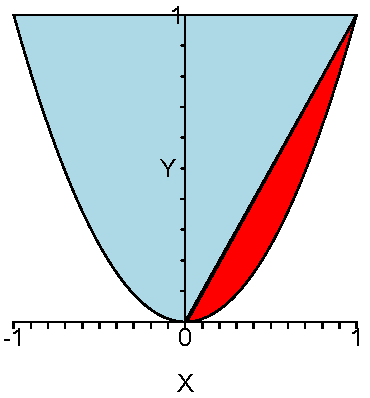
\includegraphics[width=\textwidth]{Figures/ex3-range3.pdf}
\end{center}
}
{
%{\scriptsize
\vspace{-0.5cm}\pause
\begin{align*}
\uncover<3->{P(X \geq Y) &=  \int_{0}^1 \int_{{\color{red}x^2}}^{\color{red}x} \frac{21}{4} x^2 y~{\color{red}dy}~dx \\}
            \uncover<4->{&= \frac{21}{4} \int_{0}^1 \left(\left. \frac{x^2y^2}{2}\right|_{x^2}^x\right) dx \\}
            \uncover<5->{&= \frac{21}{4} \int_{0}^1 \left(\frac{x^4}{2} - \frac{x^6}{2}\right) dx \\}
            \uncover<6->{&= \frac{21}{4} \left.\left(\frac{x^5}{10} - \frac{x^7}{14}\right)\right|_0^1 \\}
            \uncover<7->{&= \frac{21}{4} \left(\frac{1}{10} - \frac{1}{14}\right) \\}
            \uncover<8->{&= \frac{21}{4} \left(\frac{2}{70}\right)} \uncover<9->{ = 0.15}
\end{align*}
%}
}

\end{frame}

%%%%%%%%%%%%%%%%%%%%%%%%%%%%%%%%%%%%%%%%%%

\begin{frame}

\twocol{0.3}{0.7}
{
\begin{center}
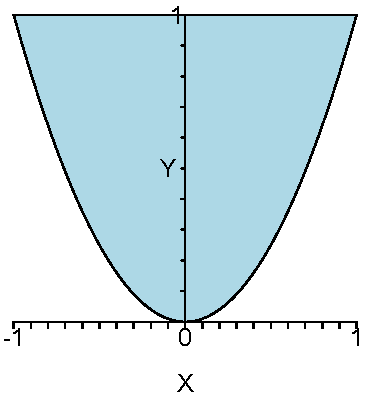
\includegraphics[width=\textwidth]{Figures/ex3-range2.pdf}
\end{center}
}
{
%{\scriptsize
\vspace{-0.5cm}
\begin{align*}
f_X(x) &= \int_{{\color{red}x^2}}^{\color{red}1} \frac{21}{4}x^2y~{\color{red}dy} \\
       \uncover<2->{&= \frac{21}{4} \left( \left. \frac{x^2y^2}{2}\right|_{x^2}^1 \right) \\}
       \uncover<3->{&= \frac{21}{8} \left( x^2 - x^6 \right),~\text{for $x \in (-1,1)$} \\ \\}
\uncover<4->{
f_Y(y) &= \int_{{\color{red}-\sqrt{y}}}^{{\color{red}\sqrt{y}}} \frac{21}{4}x^2y~{\color{red}dx} \\}
       \uncover<5->{&= \frac{21}{4} \left( \left. \frac{x^3y}{3}\right|_{-\sqrt{y}}^{\sqrt{y}} \right) \\}
       \uncover<6->{&= \frac{21}{4} \left( 2\frac{y^{5/2}}{3} \right) \\}
       \uncover<7->{&= \frac{7}{2} y^{5/2},~\text{for $y \in (0,1)$} \\}
\end{align*}
%}
}

\end{frame}

%%%%%%%%%%%%%%%%%%%%%%%%%%%%%%%%%%%%%%%%%%
\begin{frame}%\frametitle{Recap}

{\bf Joint distribution of two continuous random variables }
\begin{itemize}
\item Joint pdf
  \begin{itemize}
  \item Non-negative $f_{X, Y}(x, y) \geq 0$, for any $x, y \in \mathbb{R}$
  \item $\int_{-\infty}^{\infty} \int_{-\infty}^{\infty} f_{X, Y}(x,y) ~dx~dy = 1$
  \item For any set $C \subset \mathbb{R}^2$,
  \[ P[(X, Y) \in C] = \iint_{(x, y) \in C} f_{X, Y}(x,y) ~dx~dy\]
  \end{itemize}
\item Between joint cdf and joint pdf
\[ F_{X, Y}(a,b) = \int_{-\infty}^{b} \int_{-\infty}^{a}f_{X, Y}(x,y)~dx~dy \]
\[ f_{X, Y}(x,y) = \frac{\partial^2}{\partial x \partial y} F_{X, Y}(x,y) \]

\item Marginal pdfs
\[ f_X(x) = \int_{-\infty}^\infty f_{X, Y}(x,y)~dy, \quad f_Y(y) = \int_{-\infty}^\infty f_{X, Y}(x,y)~dx \]
\end{itemize}


\end{frame}



%%%%%%%%%%%%%%%%%%%%%%%%%%%%%%%%%%%%%%%%%%
\section{Independent random variables}
%%%%%%%%%%%%%%%%%%%%%%%%%%%%%%%%%%%%%%%%%%
\begin{frame}\frametitle{Independent random variables}
\begin{defn}
Random variables $X$ and $Y$ are \hl{independent} if any real sets $A, B \subset \mathbb{R}$,
\[P(X \in A, Y \in B) = P(X \in A) P(Y \in B)\]
\end{defn}

Random variables $X$ and $Y$ are independent {\bf if and only if}
\begin{itemize}
\item Cdf: for any $x, y \in \mathbb{R}$
\[F_{X, Y}(x, y) = F_X(x) F_Y(y)\]
\item If both are discrete, pmf: for any $x, y \in \mathbb{R}$
\[p_{X, Y}(x, y) = p_X(x) p_Y(y)\]
\item If both are continuous, pdf: for any $x, y \in \mathbb{R}$
\[f_{X, Y}(x, y) = f_X(x) f_Y(y)\]

\end{itemize}
\end{frame}

%%%%%%%%%%%%%%%%%%%%%%%%%%%%%%%%%%%%%%%%%%
\begin{frame}\frametitle{Independent random variables}

The continuous (discrete) random variables $X$ and $Y$ are independent {\bf if and only if}
their joint probability density (mass) function can be expressed as
\[f_{X, Y}(x, y) = g(x) h(y), \quad -\infty < x, y < \infty \]

\vfill

\end{frame}


%%%%%%%%%%%%%%%%%%%%%%%%%%%%%%%%%%%%%%%%%%
\begin{frame}%\frametitle{Independent random variables}
\cl{Let X and Y be drawn uniformly from the triangle below, i.e., their
joint pdf is
\[ f(x,y) = \begin{cases}
    \frac{2}{9} & \text{ for } x\geq 0, y \geq 0 \text{ and } x+y \leq 3 \\
    0           & \text{otherwise}
\end{cases}
 \]
Are they independent?
}
\twocol{0.3}{0.7}
{
\begin{center}
    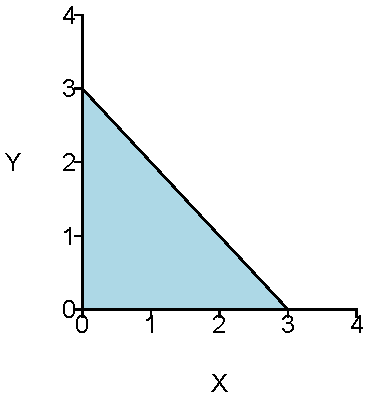
\includegraphics[width=\textwidth]{figures/triangle2.pdf}
\end{center}
}
{
\pause Denote indicator function,
\[ I(x,y) = \begin{cases}
    1 & \text{ for } x\geq 0, y \geq 0 \text{ and } x+y \leq 3 \\
    0           & \text{otherwise}
\end{cases}
 \]
\pause Then for any $x, y \in \mathbb{R}$,
$f(x, y) =  \frac{2}{9}~I(x, y)$. \\
\pause So NOT independent.\\
}
\end{frame}

\begin{frame}
We can also use marginal pdfs $f_X(x), f_Y(y)$ to double check.

\pause
$$f(x, y) = \frac{2}{9}$$ 

while for $x \in [0, 3]$ and $y \in [0, 3]$,

$$f_X(x)f_Y(y) = \frac{2}{9}(3 - x) \frac{2}{9}(3 - y) \neq \frac{2}{9}$$
\pause So NOT independent.\\
\end{frame}

%%%%%%%%%%%%%%%%%%%%%%%%%%%%%%%%%%%%%%%%%%
\begin{frame}\frametitle{More than two random variables}
\begin{dinglist}{\DingListSymbolA}
\item Random variables $X_1, X_2, \ldots, X_n$ are \hl{independent} if any real sets $A_1, A_2, \ldots, A_n \subset \mathbb{R}$,
\[P(X_1 \in A_1,  \ldots, X_n \in A_n) = P(X_1 \in A_1) \cdots P(X_n \in A_n)\]
\end{dinglist}

Random variables $X_1, X_2, \ldots, X_n$ are independent {\bf if and only if}
\begin{itemize}
\item Cdf: for any $x_1, x_2, \ldots, x_n \in \mathbb{R}$
\[F(x_1, \ldots, x_n) = F_{X_1}(x_1)\cdots F_{X_n}(x_n)\]
\item  If both are discrete, pmf: for any $x_1, x_2, \ldots, x_n \in \mathbb{R}$
\[p(x_1, \ldots, x_n) = p_{X_1}(x_1)\cdots p_{X_n}(x_n)\]
\item If both are continuous, pdf: for any $x_1, x_2, \ldots, x_n \in \mathbb{R}$
\[f(x_1, \ldots, x_n) = f_{X_1}(x_1)\cdots f_{X_n}(x_n)\]

\end{itemize}
\end{frame}



\end{document}
